\documentclass[tikz,border=10pt]{standalone}
\usetikzlibrary{arrows.meta, positioning, calc}
\usepackage[T1]{fontenc}
\usepackage{helvet}
\renewcommand{\familydefault}{\sfdefault}

\begin{document}
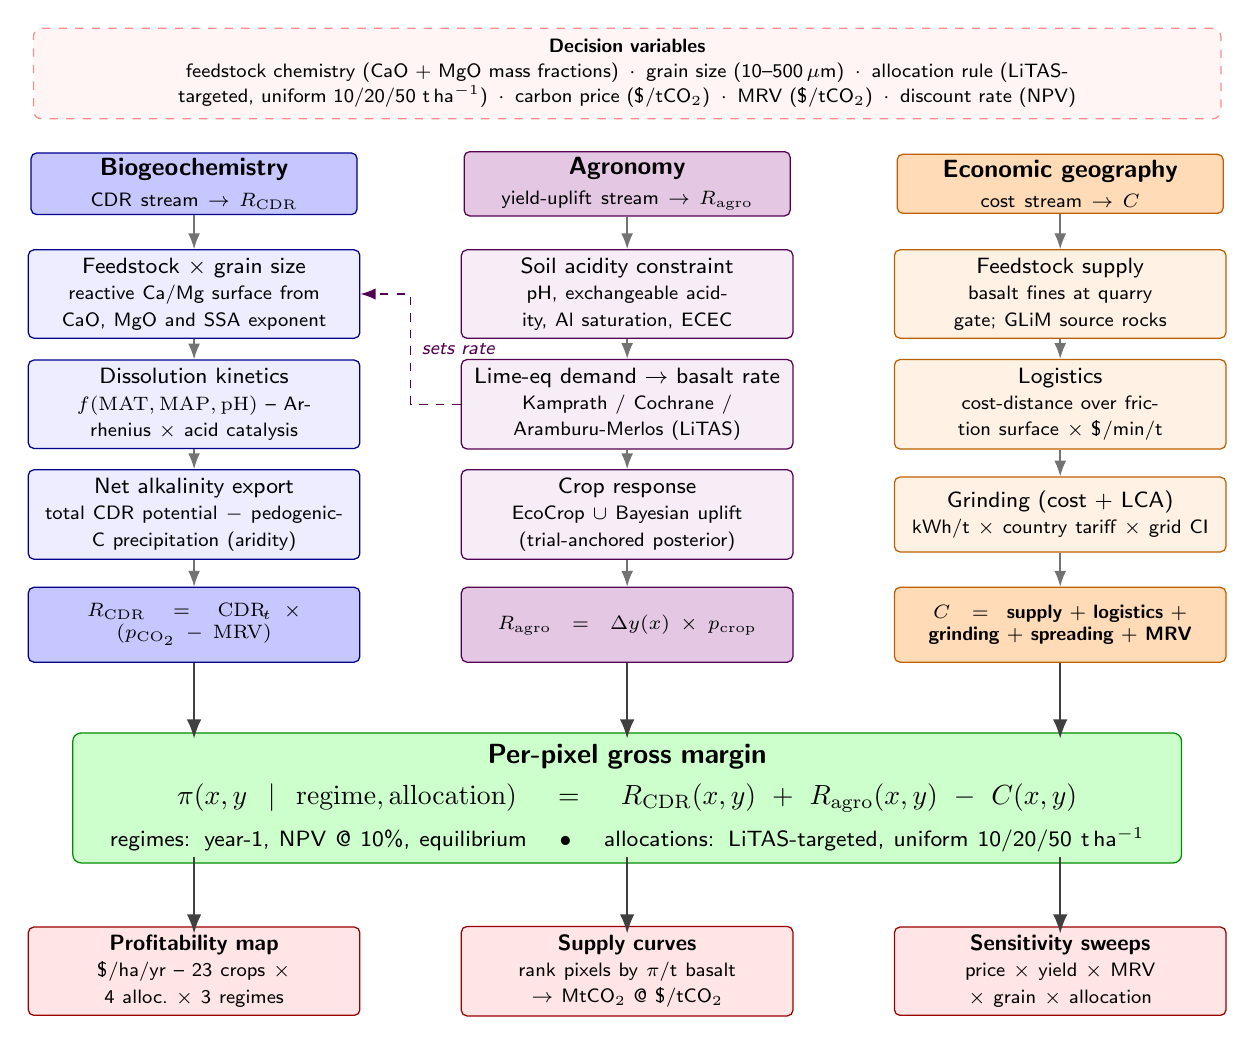
\begin{tikzpicture}[
  >=Latex,
  font=\sffamily\footnotesize,
  line width=0.45pt,
  every path/.append style={line cap=butt, line join=miter}
]

\tikzset{
  cdrhead/.style    ={draw=blue!55!black,   fill=blue!22,   rounded corners=2pt, text width=4.0cm, minimum height=0.75cm, align=center, inner sep=2pt, font=\sffamily\small\bfseries},
  cdrn/.style       ={draw=blue!55!black,   fill=blue!7,    rounded corners=2pt, text width=4.0cm, minimum height=0.95cm, align=center, inner sep=3pt},
  cdrtot/.style     ={draw=blue!55!black,   fill=blue!22,   rounded corners=2pt, text width=4.0cm, minimum height=0.95cm, align=center, inner sep=3pt, font=\sffamily\scriptsize\bfseries},
  agrohead/.style   ={draw=violet!65!black, fill=violet!22, rounded corners=2pt, text width=4.0cm, minimum height=0.75cm, align=center, inner sep=2pt, font=\sffamily\small\bfseries},
  agron/.style      ={draw=violet!65!black, fill=violet!7,  rounded corners=2pt, text width=4.0cm, minimum height=0.95cm, align=center, inner sep=3pt},
  agrotot/.style    ={draw=violet!65!black, fill=violet!22, rounded corners=2pt, text width=4.0cm, minimum height=0.95cm, align=center, inner sep=3pt, font=\sffamily\scriptsize\bfseries},
  econhead/.style   ={draw=orange!75!black, fill=orange!28, rounded corners=2pt, text width=4.0cm, minimum height=0.75cm, align=center, inner sep=2pt, font=\sffamily\small\bfseries},
  econn/.style      ={draw=orange!75!black, fill=orange!10, rounded corners=2pt, text width=4.0cm, minimum height=0.95cm, align=center, inner sep=3pt},
  econtot/.style    ={draw=orange!75!black, fill=orange!28, rounded corners=2pt, text width=4.0cm, minimum height=0.95cm, align=center, inner sep=3pt, font=\sffamily\scriptsize\bfseries},
  central/.style    ={draw=green!55!black,  fill=green!20,  rounded corners=3pt, text width=13.8cm, minimum height=1.5cm, align=center, inner sep=4pt, font=\sffamily\normalsize},
  output/.style     ={draw=red!60!black,    fill=red!10,    rounded corners=2pt, text width=4.0cm, minimum height=0.95cm, align=center, inner sep=3pt},
  dvarpanel/.style  ={draw=red!45, dashed, fill=red!4, rounded corners=3pt, text width=14.8cm, minimum height=1.0cm, align=center, inner sep=4pt, font=\sffamily\scriptsize},
  arr/.style        ={->, semithick, black!55},
  bigarr/.style     ={->, line width=0.9pt, black!75},
  crossarr/.style   ={->, line width=0.55pt, draw=violet!65!black, dashed}
}

% =========================================================
%   Conceptual framework -- three causal streams converging
%   on a per-pixel net-value equation, modulated by decision
%   variables (top panel).  Downstream uses at the bottom.
% =========================================================

% --- Decision-variable panel (top) ---
\node[dvarpanel] (dvars) at (5.5, 11.2) {%
  \textbf{Decision variables}\\[1pt]
  feedstock chemistry (CaO + MgO mass fractions) \,$\cdot$\,
  grain size (10--500\,$\mu$m) \,$\cdot$\,
  allocation rule (LiTAS-targeted, uniform 10/20/50 t\,ha$^{-1}$) \,$\cdot$\,
  carbon price (\$/tCO$_2$) \,$\cdot$\,
  MRV (\$/tCO$_2$) \,$\cdot$\,
  discount rate (NPV)
};

% --- Column headers ---
\node[cdrhead]  (h1) at ( 0.0, 9.8) {Biogeochemistry \\ {\scriptsize\normalfont CDR stream $\to$ $R_{\mathrm{CDR}}$}};
\node[agrohead] (h2) at ( 5.5, 9.8) {Agronomy \\ {\scriptsize\normalfont yield-uplift stream $\to$ $R_{\mathrm{agro}}$}};
\node[econhead] (h3) at (11.0, 9.8) {Economic geography \\ {\scriptsize\normalfont cost stream $\to$ $C$}};

% --- Column 1 : Biogeochemistry / CDR ---
\node[cdrn]   (c11) at (0.0, 8.4) {Feedstock $\times$ grain size \\ {\scriptsize reactive Ca/Mg surface from CaO, MgO and SSA exponent}};
\node[cdrn]   (c12) at (0.0, 7.0) {Dissolution kinetics \\ {\scriptsize $f(\mathrm{MAT}, \mathrm{MAP}, \mathrm{pH})$ -- Arrhenius $\times$ acid catalysis}};
\node[cdrn]   (c13) at (0.0, 5.6) {Net alkalinity export \\ {\scriptsize total CDR potential $-$ pedogenic-C precipitation (aridity)}};
\node[cdrtot] (c14) at (0.0, 4.2) {$R_{\mathrm{CDR}} \;=\; \mathrm{CDR}_{\!t} \,\times\, (p_{\mathrm{CO}_2} - \mathrm{MRV})$};

% --- Column 2 : Agronomy ---
\node[agron]   (c21) at (5.5, 8.4) {Soil acidity constraint \\ {\scriptsize pH, exchangeable acidity, Al saturation, ECEC}};
\node[agron]   (c22) at (5.5, 7.0) {Lime-eq demand $\to$ basalt rate \\ {\scriptsize Kamprath / Cochrane / Aramburu-Merlos (LiTAS)}};
\node[agron]   (c23) at (5.5, 5.6) {Crop response \\ {\scriptsize EcoCrop $\cup$ Bayesian uplift (trial-anchored posterior)}};
\node[agrotot] (c24) at (5.5, 4.2) {$R_{\mathrm{agro}} \;=\; \Delta y(x) \,\times\, p_{\mathrm{crop}}$};

% --- Column 3 : Economic geography ---
\node[econn]   (c31) at (11.0, 8.4) {Feedstock supply \\ {\scriptsize basalt fines at quarry gate; GLiM source rocks}};
\node[econn]   (c32) at (11.0, 7.0) {Logistics \\ {\scriptsize cost-distance over friction surface $\times$ \$/min/t}};
\node[econn]   (c33) at (11.0, 5.6) {Grinding (cost + LCA) \\ {\scriptsize kWh/t $\times$ country tariff $\times$ grid CI}};
\node[econtot] (c34) at (11.0, 4.2) {$C \;=\;$ supply $+$ logistics $+$ grinding $+$ spreading $+$ MRV};

% --- In-column arrows (header -> 4 boxes) ---
\foreach \src/\dst in {h1/c11, c11/c12, c12/c13, c13/c14,
                       h2/c21, c21/c22, c22/c23, c23/c24,
                       h3/c31, c31/c32, c32/c33, c33/c34} {
  \draw[arr] (\src) -- (\dst);
}

% --- Cross-column: lime demand sets the basalt rate that drives CDR ---
\draw[crossarr] (c22.west) -- (2.75, 7.0) -- (2.75, 8.4) -- (c11.east);
\node[font=\scriptsize\itshape, anchor=west, color=violet!65!black,
      fill=white, inner sep=1pt]
  at (2.85, 7.7) {sets rate};

% --- Central convergence -- gross-margin equation ---
\node[central] (gm) at (5.5, 2.0) {%
  \textbf{Per-pixel gross margin}\\[3pt]
  $\pi(x, y \mid \mathrm{regime}, \mathrm{allocation}) \;=\; R_{\mathrm{CDR}}(x,y) \,+\, R_{\mathrm{agro}}(x,y) \,-\, C(x,y)$\\[3pt]
  {\footnotesize regimes: year-1, NPV @ 10\%, equilibrium $\quad\bullet\quad$ allocations: LiTAS-targeted, uniform 10/20/50 t\,ha$^{-1}$}
};

% --- Stream totals into the gross-margin equation ---
\draw[bigarr] (c14.south) -- (0.0,  2.75);
\draw[bigarr] (c24.south) -- (5.5,  2.75);
\draw[bigarr] (c34.south) -- (11.0, 2.75);

% --- Outputs ---
\node[output] (o1) at ( 0.0, -0.2) {\textbf{Profitability map}\\{\scriptsize \$/ha/yr -- 23 crops $\times$ 4 alloc.\ $\times$ 3 regimes}};
\node[output] (o2) at ( 5.5, -0.2) {\textbf{Supply curves}\\{\scriptsize rank pixels by $\pi$/t basalt $\to$ MtCO$_2$ @ \$/tCO$_2$}};
\node[output] (o3) at (11.0, -0.2) {\textbf{Sensitivity sweeps}\\{\scriptsize price $\times$ yield $\times$ MRV $\times$ grain $\times$ allocation}};

% --- Gross margin to outputs ---
\draw[bigarr] (0.0,  1.25) -- (0.0,  0.275);
\draw[bigarr] (5.5,  1.25) -- (5.5,  0.275);
\draw[bigarr] (11.0, 1.25) -- (11.0, 0.275);

\end{tikzpicture}
\end{document}
